\section{State estimation}
\subsection{Choice of state estimation approach}
\subsection{Nonlinear observer design}

\todo{Clean up this whole thing, adding figures and such to make it less dense.}

Following the work done in ref \cite{Automatica08} and ref \cite{MainStateEst}, it was decided to implement a nonlinear observer, estimating longitudinal and lateral velocity, yaw rate, ground-tire friction coefficient, bank angle and inclination angle. \par

\subsubsection{Longitudinal velocity}
For the longitudinal velocity there are three sources of information; the rpms of the wheels, the acceleration measured by the IMU and the power used by the motors. It was decided to use the former two. Using the power from the motor might have given a better estimate of the slip ratio, but it was deemed to complex and time consuming for the allotted time. \\ 

To estimate the longitudinal velocity the following observer was used
\begin{equation}
    \dot{\hat{v}}_x = a_x + \dot{\psi}\hat{v}_y + K_{v_x}(t)(v_{x,rpm} - \hat{v}_x)
\end{equation}
where $\hat{v}_x$ is our estimate of longitudinal velocity $v_x$; $a_x$ is the measured longitudinal acceleration; $\psi$ is the yaw angle and $K_{v_x}(t)$ is a time varying gain, chosen to downweight the velocity calculated from the wheel rpms when the estimates have a high variance. $v_{x,rpm}$ is calculated as 
\begin{equation}
    v_{x,rpm} = mean(\sum_{i=1}^{4} \omega_{i}R_{eff,i}(t))
\end{equation}
where $\omega_i$ is the angular velocity of wheel i and $R_{eff,i}(t)$ is the effective wheel radius of wheel $i$ at time $t$. The wheel radius is a function of ride height only, as the expansion of the tyre due to an increase in rotational speed was deemed negligible. The wheel radius of wheel $i$ is calculated using the so called Magic Formula 5.2 for tire radius \cite{MagicFormula5_2}

\begin{equation}
    R_{eff,i}(t) = R_0 - (R_0-R_{L800N}([D_{R_{eff}}atan(B_{R_{eff}}\rho) + \\ F_{R_{eff}}\rho]
\end{equation}
with
\begin{equation}
    \rho = \frac{R_0-R_l(t)}{R_0-R_{L800N}}
\end{equation}
The coefficients $D_{R_{eff}}, B_{R_{eff}}$ and $F_{R_{eff}}$ where in the tyres datasheet, and $R_0$ and $R_{L800N}$ where found empirically. $R_0$ is the radius when unloaded, while $R_{L800N}$ is the mean of the radius of the wheel when loaded with 800N and in different angles. $R_l(t)$ is the current distance from the wheel centrum to the ground, either measured by a ride height sensor, or estimated using estimates of the wheel loads.

\subsubsection{Lateral velocity} \\
To estimate the lateral velocity, an estimate of the lateral forces is first made, by using the pure lateral magic formula 5.2 \cite{MagicFormula5_2}. This assumes that the longitudinal acceleration is negligible when cornering, but since the controller is told to never accelerate in corners, this assumption is always satisfied. The only time when the controller does accelerate when cornering is when the emergency brake has been turned on, in which case the state estimation isn't going to be used anyways and the whole system needs to be rebooted. \\ 

The magic formula gives the lateral force on each wheel in the wheel frame. These are then rotated into the body-fixed frame located in the center of gravity (CG), and summed to find the total lateral acceleration. This is done by doing the following calculation

\begin{align}
    F_y(F_{z,i},\hat{v_x},\hat{v_y},\dot{\hat{\psi}}, \theta) & = \frac{1}{\mu_{H}^{*}}\sum_{i=1}^{4}cos(\delta_i)\theta F_{y,i}(F_{z,i},\hat{v_x},\hat{v_y},\dot{\hat{\psi}}, \mu_{H}^{*}) \\
    & =  \theta F_y^{*}
\end{align}

$F_{y,i}(F_{z,i},\hat{v_x},\hat{v_y},\dot{\hat{\psi}}, \mu_{H}^{*})$ is the lateral force on wheel $i$ at the nominal value of the friction coefficient $\mu_{H}^{*}$. $\theta$ is our estimate of the friction coefficient. $F_{z,i}$ is our estimate of the vertical load on wheel $i$. $\delta_i$ is the angle of wheel $i$ with the x axis of the body frame, found by using a lookup table from the measured steering wheel angle to the wheel angle. Note that for the two rear wheels the wheel angle $\delta_i$ is always zero. \\ 

$F_{z,i}$ is found by adding together the force on the wheel when the car is standing still, with the shifted weight found by using the lateral and longitudinal acceleration measurements.  \\

The above calculation gives the lateral force, which is then divided by $(1 + p_{\phi}g)m$ to give the pure lateral acceleration. $g$ is the gravitational constant at sea level, $m$ is the mass of the vehicle and $p_{\phi}$ is the so called roll gradient, giving the relationship between the lateral acceleration and roll angle. This removes the added acceleration in the lateral direction as a result of roll angle when cornering. Calling this new estimate $a_y = \theta a_y^*$. This estimate is then used in the observer for the lateral velocity

\begin{equation}
    \dot{\hat{v}}_y = a_y - \dot{\hat{\psi}}\hat{v}_x + K_{v_y}\xi(t,\hat{x})\Lambda(a_y - \theta a_y^{*}) + \frac{\Gamma_2}{\Gamma_1}\zeta(\dot{\psi} - \dot{\hat{\psi}})
\end{equation}

where $\Gamma_1$ and $\Gamma_2$ are positive gain, $\xi(t,\hat{x})$ is a time varying gain that gives how much faith is put in the magic formula estimated acceleration. We chose
\begin{equation}
    \xi(t,\hat{x}) = \frac{\delta \hat{a}_y^*}{\delta \hat{v}_y}(t,\hat{x})
\end{equation}

$\Lambda$ is a scaling signal that prevents large variations in the gain. We chose

\begin{equation}
    \Lambda(t,\hat{x}) = (\xi^2(t,\hat{x}) + \hat{a}_y^*^2(t,\hat{x}))^{-1/2}
\end{equation}

Similarily $\zeta$ is a gain that determines how much faith we put in the yaw rate estimate determined by the wheel velocities versus the yaw rate measurement coming out of the IMU. More on this later. 

\subsubsection{Yaw rate}

To estimate the yaw rate, we have our measurement of yaw rate, but since this is noisy we would like to add one more source of information. To do this we again use the magic formula for the lateral force on the wheels, but this time use it to find the torque around the CG.
\begin{equation}
    f_r(F_{z,i}, \hat{v_x}, \hat{v_y}, \dot{\hat{\psi}}) =\theta f_r^*(F_{z,i}, \hat{v_x}, \hat{v_y}, \dot{\hat{\psi}}) 
\end{equation}
where
\begin{equation}
    f_r^*(F_{z,i}, \hat{v_x}, \hat{v_y}, \dot{\hat{\psi}}) = \frac{1}{\mu_H^*}\sum_{i=1}^{4}g_i^TR(\delta_i)F_{y,i}(F_{z,i}, \hat{v_x}, \hat{v_y}, \dot{\hat{\psi}}, \mu_H^*)
\end{equation}
with 

\begin{equation}
    g_i = \begin{bmatrix} -l_i sin(\alpha_i) \\ h_i cos(\alpha_i)
    \end{bmatrix}
\end{equation}
where for convenience it has been defined

\begin{align}
    \alpha_1 & = -\gamma_1 \\
    \alpha_2 & = \gamma_2 \\
    \alpha_3 & = \pi + \gamma_3 \\
    \alpha_4 & = \pi -\gamma_4 \\
\end{align}

The $l_i$'s are the lengths from the CG to the wheel $i$, while the $\gamma_i$'s are the angles the line going through both CG and wheel $i$ make with the longitudinal axis of the car. This is more easily understood by lookin at figure \ref{Fig:WheelTorques}. \\

\begin{figure}
    \centering
    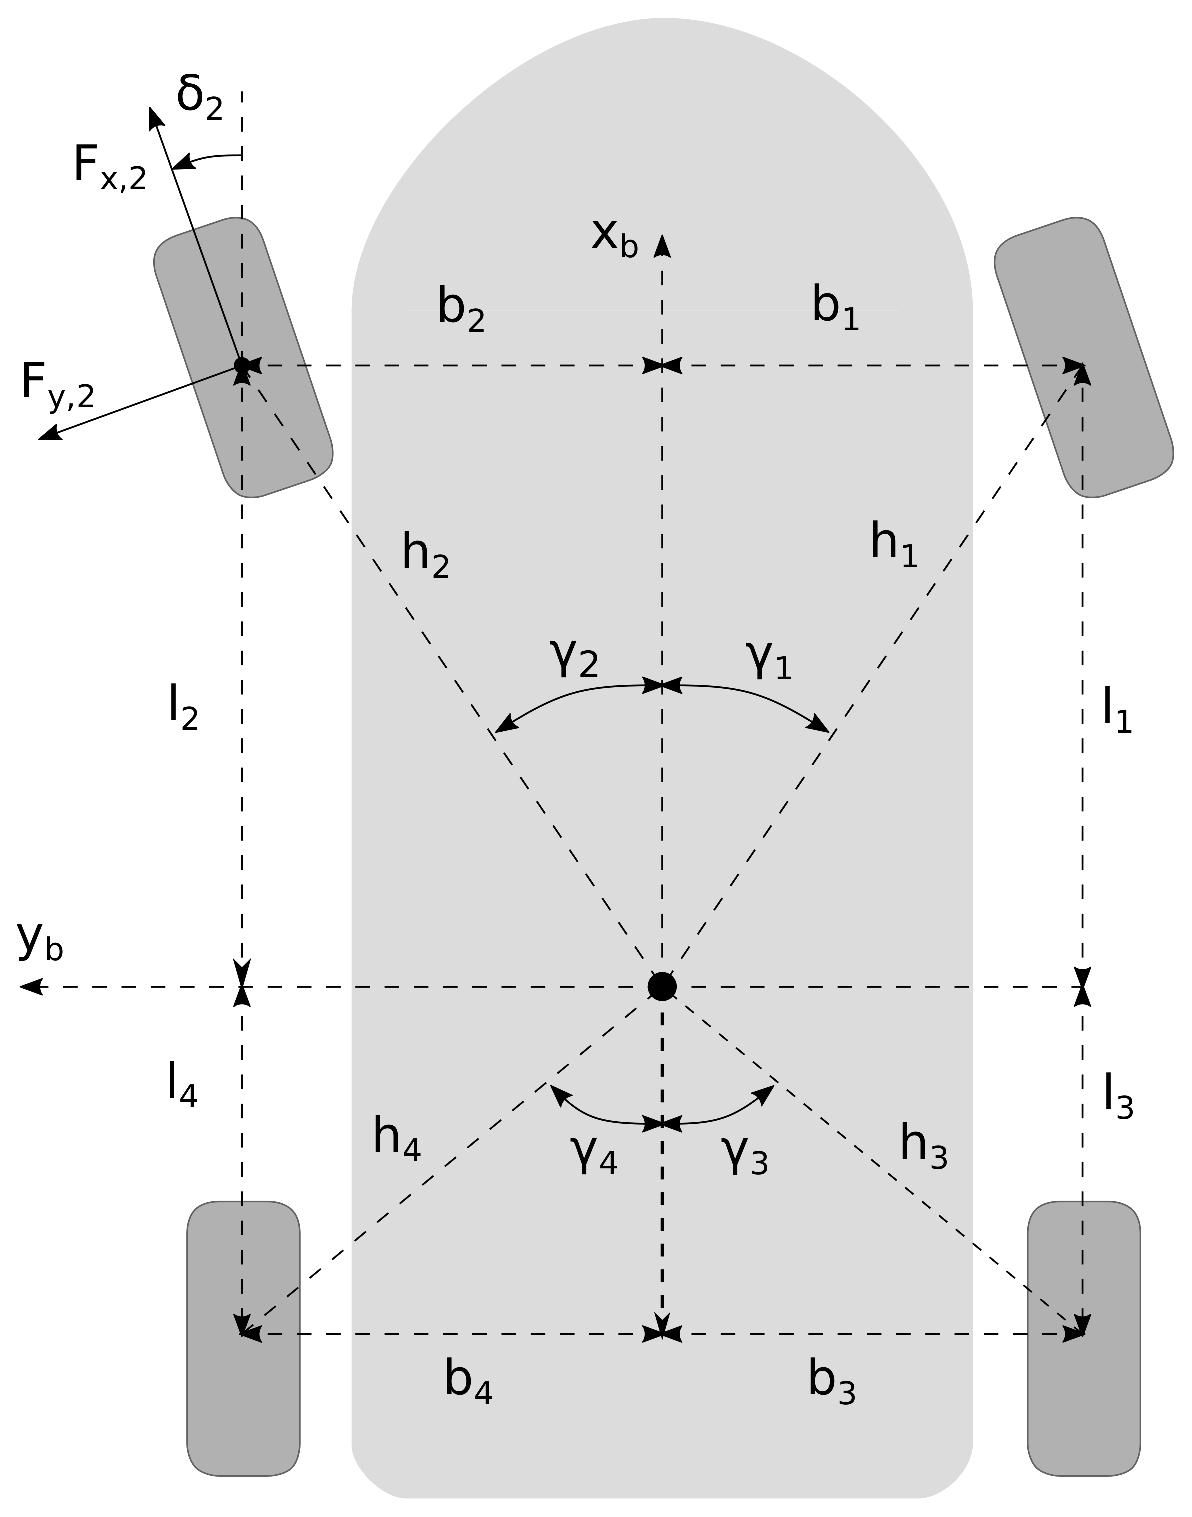
\includegraphics[width=0.5\linewidth]{0_Images/3_Theory/TorqueCalculations.eps}
    \captionof{figure}{Illustrations of variables used for torque calculations.}
    \label{Fig:WheelTorques}
\end{figure}

This estimate is then used in much the same way as for the longitudinal velocity to update our estimate of the yaw rate.

\begin{equation}
    \ddot{\hat{\psi}} = \frac{1}{J}\theta \hat{f}_r^* + k_r(\dot{\psi}-\hat{\dot{\psi}})
\end{equation}

where $J$ is the moment of intertia of the vehicle around CG, and $K_r$ is our faith in the estimate calculated by looking at lateral tyre forces, compared to yaw rate coming out of the IMU. 

\subsubsection{Friction parameter}
Instead of estimating the friction parameter directly, which would have meant one friction coefficient per wheel, we parametrize the lateral force as we have seen earlier

\begin{equation}
    f_y(F_{z,i}, \hat{v_x}, \hat{v_y}, \dot{\hat{\psi}}) =\theta f_y^*(F_{z,i}, \hat{v_x}, \hat{v_y}, \dot{\hat{\psi}}) 
\end{equation}

This is an acceptable simplification, since the formula student track is uniform tarmac without any oil spill or similar. It will only ever change friction coefficient as a result of weather, and then it's reasonable to assume it's going to affect the track evenly since no parts are going to be under a roof. \\ 

The estimate for the simplified friction coefficient is updated using the following observer

\begin{equation}
    \dot{\theta} = K_{\theta}\Lambda (t, \hat{x})\hat{a}_y^*(t,\hat{x})(a_y - \hat{a}_y(t,\hat{x},\theta))
\end{equation}

\subsubsection{Bank and inclination angle}

The final part of the puzzle is estimating the bank and inclination angle so their effect on the lateral and longitudinal forces can be corrected for. We define the tilt of the ground as first an inclination angle $\Theta$ around the vehicles y axis, and then a bank angle $\Phi$ around the now rotated x axis. This leads to the following effect on the dynamics of the car

\begin{align}
    \dot{v}_x & = a_x + \dot{\psi} v_y + g sin(\Theta) \\
    \dot{v}_y & = a_y - \dot{\psi}v_x - g cos(\Theta) sin(\Phi)
\end{align}

We define $\theta_i = sin(\Theta)$ and $\theta_b = cos(\Theta)sin(\Phi)$ and assuming that the bank and inclination angles are small, these are approximately 

\begin{align}
    \theta_i & \approx \Theta \\
    \theta_b & \approx \Phi
\end{align}

We introduce an estimate of $\theta_i$ and $\theta_b$ as

\begin{align}
    \dot{\hat{\theta}}_i & = K_{\theta_i}K_{v_x}(t)(v_{x,rpm} - \hat{v}_x) \\
    \dot{\hat{\theta}}_b & = K_{\theta_b}(a_y-\hat{a}_y(t,\hat{x},\theta)
\end{align}

Where $K_{v_X}$ is, as previously defined, how much faith is put in the longitudinal velocity estimate coming from the wheel RPMs. $K_{\theta_i}$ and $K_{\theta_b}$ are tuning parameters. The observers for $v_y$ and $v_x$ are modified to correct for this bias by adding $g\hat{\theta}_i$ to $\dot{\hat{v}}_x$ and $-g\hat{\theta}_b$ to $\dot{\hat{v}}_y$. 

\subsubsection{When to estimate friction}

Estimating the bank angle and estimating the friction coefficient $\theta$ are conflicting problems, as both are not properly observable at the same time. In \cite{MainStateEst} this is solved by turning of the friction coefficient update when there isn't enough lateral acceleration for it to converge properly, and turning of the bank angle update when estimating updating the friction coefficient. They found that this worked well in most cases, but that when driving in terrain that is both hilly, meaning varying bank angle, and with a low friction coefficient, they needed to estimate both at the same time. \\

To do this they developed a rather complex set of rules for when to turn on and of the two different update laws. We believe this is not needed in our case, since we are driving on flat ground with a slowly varying bank angle and a friction coefficient that never goes down as low as theirs did. They were driving on snow and ice, while the worst condition we will face will be wet tarmac, so as long as we estimate the bank angle regularly, there shouldn't be a need to estimate both bank angle and friction coefficient at the same time. \\

We therefore employ the same switching rule for when to update the friction coefficient as \cite{MainStateEst} and simply turn of the bank angle update when friction coefficient is being updated. To determine when to turn on the friction update we estimate the reference yaw rate found by looking at the wheel torques, and an estimate of $\dot{v}_y$. $\dot{\hat{v}}_y$ found by low pass filtering $a_y - \dot{\psi}\hat{v}_x$. A high value for $\dot{v}_y$ indicates a high level of excitation and that some of the tyres might be in the nonlinear region where it's possible to get information about the friction coefficient. When both these values are high enough we turn on friction update and turn off bank angle update. \\ 

Ref. \cite{MainStateEst} lets the friction coefficient go exponentially to a nominal value of 1 when it isn't being estimated from the sensor data. They argue that dry tarmac will be the normal operating conditions. We chose instead to simply let the coefficient stay at that value when we aren't updating it from the sensor data, seeing how the ground conditions will change rather slowly.

\subsubsection{Final observer}
The full observer has to modes: either it updates the estimate of the bank angle, or it updates the estimate of the friction coefficient. In the first case the full observer is as follows

\begin{align}
    \dot{\hat{v}}_x & = a_x + \dot{\hat{\psi}}\hat{v}_y + g\hat{\theta}_i + K_{v_x}(t)(v_{x,rpm} - \hat{v}_x) \\
    \dot{\hat{v}}_y & = a_y - \dot{\hat{\psi}}\hat{v}_x - g\hat{\theta}_b + K_{v_y}\xi(t,\hat{x})\Lambda(a_y - \theta a_y^{*}) + \frac{\Gamma_2}{\Gamma_1}\zeta(\dot{\psi} - \dot{\hat{\psi}}) \\ 
    \dot{\hat{\theta}}_i & = K_{\theta_i}K_{v_x}(t)(v_{x,rpm} - \hat{v}_x) \\
    \dot{\hat{\theta}}_b & = K_{\theta_b}(a_y-\hat{a}_y(t,\hat{x},\theta)) \\ 
    \ddot{\hat{\psi}} & = \frac{1}{J}\theta \hat{f}_r^* + k_r(t)(\dot{\psi}-\hat{\dot{\psi}})
\end{align}

When updating friction coefficient and not bank angle the observer looks like this

\begin{align}
    \dot{\hat{v}}_x & = a_x + \dot{\psi}\hat{v}_y + g\hat{\theta}_i + K_{v_x}(t)(v_{x,rpm} - \hat{v}_x) \\
    \dot{\hat{v}}_y & = a_y - \dot{\hat{\psi}}\hat{v}_x - g\hat{\theta}_b + K_{v_y}\xi(t,\hat{x})\Lambda(a_y - \theta a_y^{*}) + \frac{\Gamma_2}{\Gamma_1}\zeta(\dot{\psi} - \dot{\hat{\psi}}) \\ 
    \dot{\hat{\theta}}_i & = K_{\theta_i}K_{v_x}(t)(v_{x,rpm} - \hat{v}_x) \\
    \dot{\theta} & = K_{\theta}\Lambda (t, \hat{x})\hat{a}_y^*(t,\hat{x})(a_y - \hat{a}_y(t,\hat{x},\theta)) \\ 
    \ddot{\hat{\psi}} & = \frac{1}{J}\theta \hat{f}_r^* + k_r(t)(\dot{\psi}-\hat{\dot{\psi}})
\end{align}

Uniform Global Asymptotical Stability (UGAS) and Uniform Local Exponential Stability (ULES) of the error of the estimator for $(v_x,v_y,r,\theta)$ was proven in \cite{Automatica08}, while UGAS of the error for the estimator for $(v_x,v_y,\theta, \theta_i, \theta_b)$ was proven in \cite{MainStateEst}. The first of these implies UGAS and UGES of the full observer of $(v_x,v_y, r,\theta, \theta_i, \theta_b)$, as long as the gains on the bank and inclination angle estimates are small enough, and the estimates of $\theta$, $\theta_i$ and $\theta_b$ are limited to a small enough range. This is because UGAS together with ULES implies a certain robustness to small constant biases, which is the effect a wrong estimate of the bank and inclination angles would add to the update laws for $\hat{v}_x$ and $\hat{v}_y$. 
